\newpage
\section{Transportschicht}
  \subsection{Grundlagen}
    \begin{itemize}
      \item Datenaustausch zwischen Anwendungsprozesse
        \begin{itemize}
          \item Nutzer-zu-Nutzer Kommunikation
          \item Pakete werden hier typischerweise als Segmente oder Datagramme bezeichnet
          \item Transportprotokolle sind in Systemen lokalisiert auf denen sich Anwendungsprozesse
            befinden, also Endsysteme
        \end{itemize}
      \item Eigenschaften
        \begin{itemize}
          \item Verbergen von Details des Datentransports vor höheren Schichten
            \begin{itemize}
              \item Fehlercharakteristika
              \item Genutzte Technologien
              \item ...
            \end{itemize}
          \item ... nicht alles lässt sich verbergen
            \begin{itemize}
              \item Verzögerung bleibht "sichtbar"
              \item Schwerwiegende Fehler ebenfalls "sichtbar"
            \end{itemize}
          \item Aufgaben
            \begin{itemize}
              \item Adressierung von Anwendungsprozessen
              \item Multiplexen / Demultiplexen
              \item Bereitstellung zuverlässiger und unzuverlässiger Transportdienste
                \begin{itemize}
                  \item Fehlererkennung und -behebung für zuverlässige Transportdienste
                  \item Pufferung der Daten in den Endsystemen für zuverlässige Transportdienste
                \end{itemize}
              \item Segmente/Datagramme der Transportschicht werden in ein oder mehreren Datagrammen
                der Vermittlungsschicht übertragen
            \end{itemize}
        \end{itemize}
    \end{itemize}
    \subsubsection{Nutzer-zu-Nutzer versus Ende-zu-Ende}
      Beispiel: Senden von Briefen mittels traditioneller Post
      \begin{itemize}
        \item Brief: Anwendugnsnachricht
        \item Kommunikation zwischen Häusern (Endsystemen)
          \begin{itemize}
            \item Ende-zu-Ende (zwischen Briefkästen)
          \end{itemize}
        \item Bob leert Briefkasten (Demultiplexen der Briefe auf Bewohner)
          \begin{itemize}
            \item Bob ist im Haus (also Endsystem)
          \end{itemize}
        \item Kommunikation zwischen Bewohnern (Anwendungsprozessen)
          \begin{itemize}
            \item Nutzer-zu-Nutzer (die einzelnen Briefe)
          \end{itemize}
        \item Bob wirft zu sendenden Brief in Briefkasten (Multiplexen der Briefe der Bewohner)
      \end{itemize}
    \subsubsection{Transportprotokolle im Internet}
      Im wesentlichen
      \begin{itemize}
        \item UDP (User Datagramm Protocol)
          \begin{itemize}
            \item Bietet unzuverlässigen Transportdienst
          \end{itemize}
        \item TCP (Transmission Control Protocol)
            \begin{itemize}
              \item Bietet zuverlässigen Transportdienst
            \end{itemize}
      \end{itemize}
  \subsection{Client-Server Architektur}
    \begin{itemize}
      \item Ein Server ist ein System welches ständig betriebsbereit und erreichbar ist und erreichbar ist
        und vielen anderen Systemen, genannt Clients, Dienste bereitstellt
      \item Haben i.d.R. statische IP-Adresse
      \item I.d.R. leistungsfähige Hardware
        \begin{itemize}
          \item Oft in Rechnerzentren plaziert
        \end{itemize}
      \item Ein Client ist ein System, welches Dienste auf einem Server in Anspruch nimmt. Client ist
        evtl. nicht immer in Betrieb oder erreichbar
        \begin{itemize}
          \item Standby, dynamische IP-Adresse ...
        \end{itemize}
      \item Kommuniziert nur mit Server, nicht direkt mit anderen Clients
    \end{itemize}
  \subsection{Adressierung}
    \subsubsection{Adressierung auf Transportschicht}
      Ziel
      \begin{itemize}
        \item Eindeutige Identifikation der Nutzer (Anwendungsprozess) in einem Endsystem
        \item Ermöglicht Multiplexing/Demultiplexing auf Endsystemen
          \begin{itemize}
            \item Viele Anwendugnsprozesse auf dem Endsystem kommunizieren gleichzeitig über das Netz
              mit Anwendungsprozessen auf entfernten Endsystemen
          \end{itemize}
      \end{itemize}
      Ports
      \begin{itemize}
        \item Adressen der Transportschicht
        \item Unstrukturierte Nummer der Länge 16 Bit
        \item Lokal (im Endsystem) eindeutig
        \item Viele Portnummern kleiner 1024 für häufig benutzte Anwendungen reserviert (well-known
          ports)
      \end{itemize}
    \subsubsection{Vergabe von Portnummern}
      Well-known ports oder system ports (0 - 1023)
      \begin{itemize}
        \item Vergabe durch IANA (Internet Assigned Numbers Authority)
        \item Nutzung nur durch Systemprozesse oder privilegierte Prozesse
      \end{itemize}
      Registered ports oder user ports (1024 - 49151)
      \begin{itemize}
        \item Registrierung durch IANA
        \item Nutzung durch Nutzerprozesse ohne besondere Rechte
      \end{itemize}
      Dynamic pors oder private ports (4912 - 65535)
      \begin{itemize}
        \item Keine Registrierung vorgesehen
      \end{itemize}
  \subsection{UDP}
    Überblick
    \begin{itemize}
      \item Sehr einfaches Transportprotokoll
        \begin{itemize}
          \item RFC 768, August 1980
        \end{itemize}
      \item Eigenschaften
        \begin{itemize}
          \item Multiplexen / Demultiplexen von Datagrammen für Anwendungsprozesse
          \item Überprüfung von Bitfehlern: Prüfsumme
          \item Bietet unzuverlässigen Transportdienst an
        \end{itemize}
      \item UDP-Datagramm\\
        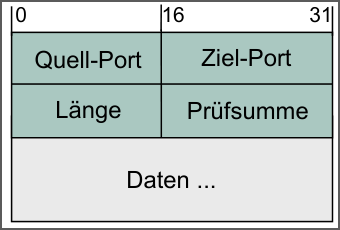
\includegraphics[width=.4\textwidth]{img/udp_datagramm.png}
    \end{itemize}
  Eigenschaften von UDP
    \begin{itemize}
      \item Geringe Overhead durch Transportkopf
        \begin{itemize}
          \item 8 Byte: Ports, Längenfeld und Prüfsumme
        \end{itemize}
      \item Unreguliertes Senden
        \begin{itemize}
          \item UDP kann Daten so schnell senden, wie sie von der Anwendung geliefert und vom Netz
            abgenommen werden
        \end{itemize}
      \item Best Effort (unzuverlässiger Transportdienst)
        \begin{itemize}
          \item Keine Zusagen über Auslieferung der Daten beim Empfänger
        \end{itemize}
      \item Keine Verbindungsaufbauphase
        \begin{itemize}
          \item Daten können sofort gesendet werden, keine "Vorarbeiten" erforderlich
          \item Damit keine zusätzliche Verzögerung
        \end{itemize}
      \item Kein Verbindungszustand
        \begin{itemize}
          \item Keine verbindungsrelevanten Informationen im Endsystem
            \begin{itemize}
              \item z.B. Flusskontrollfenster, Sequenznummern, Zeitgeber
            \end{itemize}
          \item Skaliert z.B. für Server besser
            \begin{itemize}
              \item Können mit UDP typischerweise mehr Kommunikationsbeziehungen unterstützen als mit
                TCP
            \end{itemize}
        \end{itemize}
      \item Keine Verbindungsabbauphase
        \begin{itemize}
          \item Es müssen nach dem Senden der Daten keine Zustände gelöscht werden
        \end{itemize}
    \end{itemize}
    Internet-Prüfsumme
    \begin{itemize}
      \item Prüfsumme bei Internet-Protokollen
        \begin{itemize}
          \item Speziell für Realisierung in Software ausgelegt
          \item Verwendet bei: UDP, TCP und IPv4
        \end{itemize}
      \item Prinzip
        \begin{itemize}
          \item Aufaddieren aller übertragenen Wörter (16 Bit Wortlänge)
            \begin{itemize}
              \item Wörter werden als \verb!Integer! aufgefasst
              \item Prüfsumme = $\sum$ aller übertragenen Wörter
            \end{itemize}
          \item Prüfsumme wird im Paket übertragen
        \end{itemize}
      \item Implementierung
        \begin{itemize}
          \item Addition unter Verwendung des Einer-Komplements
          \item RFC 1071: Hinweise und Techniken für effiziente Implementierung
        \end{itemize}
    \end{itemize}
    Internet-Prüfsumme bei UDP
    \begin{itemize}
      \item Prüfsumme wird berechnet über
        \begin{itemize}
          \item UDP-Kopf(Prüfsummenfeld inst initial mit 0 zu belegen)
          \item UDP-Daten
          \item Pseudoheader    
        \end{itemize}
      \item Mit IPv4
        \begin{itemize}
          \item Berechnung ist optional und kann deaktiviert werden
          \item Prüfsummenfeld = 0 : keine Prüfsummenberechnung gewünscht
          \item Bei berechneter Prüfsumme 0 wird \verb!0xFFFF! übertragen
        \end{itemize}
      \item Mit IPv6
        \begin{itemize}
          \item Berechnung verpflichtend, da sich im IPv6-Kopf keine Prüfsumme mehr befindet
        \end{itemize}
    \end{itemize}
    Pseudoheader
    \begin{itemize}
      \item Aufbau
        \begin{itemize}
          \item Quell-/Ziel-IP-Adresse
          \item Protokoll
          \item Länge des UDP-Datagramms
        \end{itemize}
        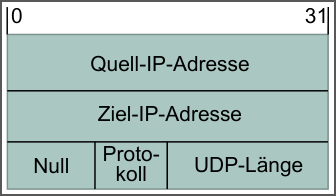
\includegraphics[width=.4\textwidth]{img/udp_pseudoheader.png}
      \item Pseudoheader wird nicht übertragen
      \item Aufgabe
        \begin{itemize}
          \item Fehler in IP-Adressen können erkannt werden, damit Schutz gegen fehlgeleitete
            UDP-Datagramme
        \end{itemize}
    \end{itemize}
    UDP-Prüfsumme
    \begin{itemize}
      \item Sender
        \begin{itemize}
          \item Datagramm (inkl. Kopf und Pseudoheader) als Folge von 16-Bit-Wörtern aufgefasst
          \item Berechnung der Prüfsumme
          \item Ergebnis in Feld Prüfsumme im UDP-Kopf eintragen
        \end{itemize}
      \item Empfänger
        \begin{itemize}
          \item Prüfsumme $P_b$ des empfangenden UDP-Datagramms berechnen
          \item Berechne Prüfsumme $P_b$ mit empfangenr Prüfsumme $P_e$ im Feld Prüfsumme vergleichen
            \begin{itemize}
              \item Werte ungleich $\ra$ Fehler erkannt
              \item Werte gleich $\ra$ kein Fehler erkannt
            \end{itemize}
        \end{itemize}
    \end{itemize}
    \subsubsection{Verteilte Anwendungen über UDP programmieren - Sockets}
      \begin{itemize}
        \item Eine verteilte Anwendung ist ein Anwendungsprogramm, das auf mehrere Endsystemen
          ausgeführt wird. Die Anwendungsprozesse auf den Endsystemen nutzen Rechnernetzte zum Austausch
          von Nachrichten
          \begin{itemize}
            \item Prozesse auf gleichem Endsystem kommunizieren vie Inter Process Communication (IPC).
              Dies ist durch das Betriebssystem geregelt.
          \end{itemize}
      \end{itemize}
      Client-Server-Anwendungen
      \begin{itemize}
        \item Eine verteilte Anwendung ist eine Client-Server-Anwendung, wenn die Anwendungsprozesse
          entweder Clientprozesse oder Serverprozesse sind.
          \begin{itemize}
            \item Serverprozesse sind ständig in Betrieb
            \item Clientprozesse senden Aufträge/Anfragen (Request) an Serverprozesse (werden dort
              bearbeitet)
            \item Serverprozesse senden Antwort (Response) an Clientprozesse zurück
            \item Clientprozesse kommunizieren nicht direkt miteinander
          \end{itemize}
      \end{itemize}
      Socket-Interface
      \begin{itemize}
        \item Programmschnittstelle für Client-Server-Anwendungen
          \begin{itemize}
            \item Application Programming Interface (API)
            \item Lokalisiert zwischen Anwendungssschicht und Transportschicht
            \item Bereitgestellt vom Betriebssystem
            \item Anwendungsprozess sendet/empfängt Daten zum/vom Socket
          \end{itemize}
      \end{itemize}
      Sockts: Eigenschaften
      \begin{itemize}
        \item Werden von Anwendungen erzeugt, genutzt und wieder freigegeben
          \begin{itemize}
            \item Adressierung auf Anwendugnsschicht über Protnummern
          \end{itemize}
        \item Ermöglicht das Lesen und Schreiben von Daten
          \begin{itemize}
            \item Interne Adressierung erfolgt über Deskriptoren
              \begin{itemize}
                \item Ablauf analog zu einfachem Dateizugriff (Filedescriptor)
                \item Transfer der Daten lokal oder über Netz
              \end{itemize}
          \end{itemize}
        \item Können empfangene oder zu sendende Daten kurzzeitig puffern
          \begin{itemize}
            \item Sende- und Empfangspuffer $\ra$ Sockets belegen Ressourcen
          \end{itemize}
        \item Basieren auf Client-Server-Architektur
          \begin{itemize}
            \item Es gibt Client-Sockt und Server-Sockets
          \end{itemize}
      \end{itemize}
  \subsection{TCP}
    \subsubsection{Grundlegendes und TCP-Segment}
      Transmission Control Protocol (TCP)
      \begin{itemize}
        \item Stellt zuverlässigen Transportdienst zur Verfügung
        \item Erhält von Anwedungsprozessen Bytestrom, übergibt an IP TCP-Segmente
      \end{itemize}
      Bytestrom $\ra$ TCP-Segment?
      \begin{itemize}
        \item Problem
          \begin{itemize}
            \item Wann wird aus Bytestrom ein TCP-Segment an IP weitergegeben?
            \item "TCP should send that data in segments at its own convenience
          \end{itemize}
        \item Alternativen
          \begin{itemize}
            \item MSS: Maximum Segment Size
              \begin{itemize}
                \item Länge der Anwendungsdaten, nicht Länge des TCP-Segments
                \item Typische Größen (vermeiden das Fragmentieren durch IP) (1460 Byte, 536 Byte
              \end{itemize}
            \item Push (PSH-Flag im Kopf des TCP-Segments)
              \begin{itemize}
                \item Sender verlangt sofortiges Versenden der Daten (Vorrangdaten)
              \end{itemize}
            \item Zeitgeber
              \begin{itemize}
                \item Nach Zeitintervall der Inaktivität werden vorhandene Daten gesendet
              \end{itemize}
          \end{itemize}
      \end{itemize}
      Zu den Eigenschaften von TCP
      \begin{itemize}
        \item Verbindungsorientierter, zuverlässiger Dienst
          \begin{itemize}
            \item Phasen: Verbindungsaufbau, Datentransfer, Verbindungsabbau
          \end{itemize}
        \item Fehlerkontrolle
          \begin{itemize}
            \item Sequenznummern, Prüfsumme, Quittierung, Sendewiederholung, Timer
          \end{itemize}
        \item Flusskontrolle (um Empfänger nicht zu überlasten)
        \item Staukontrolle (um Netz nicht zu überlasten)
      \end{itemize}
      TCP-Sequenznummern und -Quittungen
